\documentclass{standalone}
\usepackage[utf8]{inputenc}
\usepackage{tikz}
\usetikzlibrary{arrows,automata}
\usepackage{contour}
\contourlength{1pt}
\contournumber{100}

\begin{document}
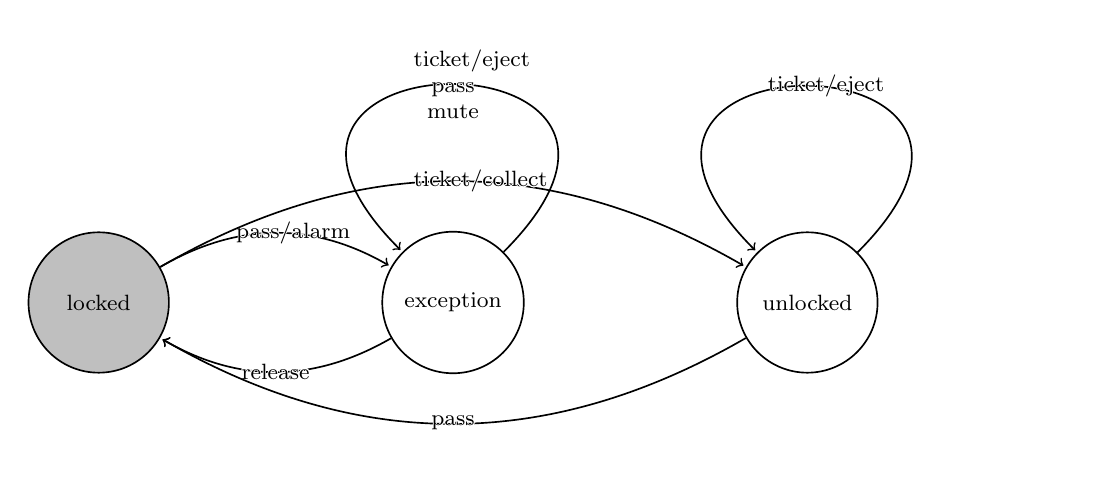
\begin{tikzpicture}[->,shorten >=1pt,node distance=4.5cm, semithick]

\tikzstyle{initial}=[fill=gray!50!white,text=black]
\tikzstyle{every node}=[font=\footnotesize]

\node[initial,state](locked){\parbox{1.5cm}{\centering locked}};
\node[state](exception)[right of=locked]{\parbox{1.5cm}{\centering exception}};
\node[state](unlocked)[right of=exception]{\parbox{1.5cm}{\centering unlocked}};


\path(exception)edge[loop]node{\parbox{1cm}{\centering \contour{white}{ticket/eject} \contour{white}{pass} \contour{white}{mute} }}(exception)
(exception)edge[bend left]node{\parbox{1cm}{\centering \contour{white}{release} }}(locked)
(locked)edge[bend left]node{\parbox{1cm}{\centering \contour{white}{pass/alarm} }}(exception)
(locked)edge[bend left]node{\parbox{1cm}{\centering \contour{white}{ticket/collect} }}(unlocked)
(unlocked)edge[bend left]node{\parbox{1cm}{\centering \contour{white}{pass} }}(locked)
(unlocked)edge[loop]node{\parbox{1cm}{\centering \contour{white}{ticket/eject} }}(unlocked)
;

\end{tikzpicture}
\end{document}
